\documentclass[11pt]{article}
\usepackage[margin=0.8in]{geometry}
\usepackage[utf8]{inputenc}
\usepackage{graphicx}
\usepackage{booktabs}
\usepackage{array}
\usepackage{multirow}
\usepackage{amsmath}
\usepackage{placeins}
\usepackage[font=small,skip=6pt]{caption}
\usepackage{subcaption}
\usepackage{microtype}
\usepackage{url}
\usepackage{iftex}
\ifXeTeX
  % XeTeX (tectonic): OpenType Times/Helvetica clones, matching main.tex
  \usepackage{fontspec}
  \setmainfont{texgyretermes}[Extension=.otf, UprightFont=*-regular, BoldFont=*-bold,
    ItalicFont=*-italic, BoldItalicFont=*-bolditalic]
  \setsansfont{texgyreheros}[Extension=.otf, UprightFont=*-regular, BoldFont=*-bold,
    ItalicFont=*-italic, BoldItalicFont=*-bolditalic]
\else
  \usepackage{mathptmx}
\fi
\urlstyle{same}
% Same figure lookup as main.tex: uploaded copies first, then the notebook outputs in place.
\graphicspath{{figures/}{../../Notebooks/}}
\captionsetup{labelfont=bf,justification=centering}
\renewcommand{\arraystretch}{1.08}
\setlength{\parskip}{6pt}
\setlength{\parindent}{0pt}
\renewcommand{\thetable}{S\arabic{table}}
\renewcommand{\thefigure}{S\arabic{figure}}
\renewcommand{\topfraction}{0.95}
\renewcommand{\textfraction}{0.05}
\renewcommand{\floatpagefraction}{0.8}
\newcommand{\panel}[3]{\begin{subfigure}[t]{#1\linewidth}\centering\includegraphics[width=\linewidth]{#2}\caption{#3}\end{subfigure}}
% One figure per model with its binary and multiclass Grad-CAM galleries.
\newcommand{\gradcamfigure}[2]{%
\begin{figure}[htbp]
\centering
\panel{1.0}{binary-detection/plots/13_gradcam_#1.png}{Binary detection.}\\[4pt]
\panel{1.0}{classification/plots/13_gradcam_#1.png}{Subtype classification.}
\caption{Grad-CAM maps of \textbf{#2} on its most confident correct and most confident wrong test predictions, from the fold with the lowest validation loss.}
\end{figure}}

\begin{document}

\begin{center}
{\Large\bfseries Supplementary Material}\\[6pt]
{\large Standardised Comparison of Convolutional and Transformer Backbones for Brain Tumour MRI Classification under Perceptual-Hash Deduplication}\\[6pt]
Parth Mital, Ved Lawand, Biji C. L., Muzaffar Ahamad Dar, George Priya Doss C.
\end{center}

This document accompanies the main manuscript. Every value is taken from the outputs of the two notebooks released with the code repository (\path{Materials/Notebooks/binary-detection} and \path{Materials/Notebooks/classification}); the source file is named in each caption. Unless stated otherwise, binary detection is evaluated on 171 held-out test images and subtype classification on 45.

\section*{S1. Data, deduplication and splitting}

\begin{table}[htbp]
\centering
\caption{Images kept by the label-aware perceptual-hash pass at each Hamming tolerance (\texttt{deduplication\_threshold\_sweep.csv}). The study uses tolerance 5. The multiclass count at tolerance 5 is before the label-noise exclusion, which brings the pool to 4,730.}
\small
\begin{tabular*}{\textwidth}{@{\extracolsep{\fill}}lccccccc@{}}
\toprule
Tolerance & 0, 1 & 2, 3 & 4, 5 & 6, 7 & 8, 9 & 10, 11 & 12 \\
\midrule
Binary, tumour-negative & 860 & 583 & 455 & 395 & 341 & 310 & 285 \\
Binary, tumour & 1,217 & 912 & 730 & 607 & 541 & 494 & 424 \\
\textbf{Binary, total} & \textbf{2,077} & \textbf{1,495} & \textbf{1,185} & \textbf{1,002} & \textbf{882} & \textbf{804} & \textbf{709} \\
\midrule
Multiclass, glioma & 2,303 & 2,221 & 2,010 & 1,653 & 1,277 & 919 & 627 \\
Multiclass, meningioma & 1,518 & 1,453 & 1,316 & 1,130 & 935 & 704 & 506 \\
Multiclass, pituitary & 1,751 & 1,663 & 1,408 & 1,145 & 886 & 663 & 478 \\
\textbf{Multiclass, total} & \textbf{5,572} & \textbf{5,337} & \textbf{4,734} & \textbf{3,928} & \textbf{3,098} & \textbf{2,286} & \textbf{1,611} \\
\bottomrule
\end{tabular*}
\end{table}

\begin{figure}[htbp]
\centering
\panel{1.0}{binary-detection/plots/01_dataset_overview.png}{Binary detection.}\\[4pt]
\panel{1.0}{classification/plots/01_dataset_overview.png}{Subtype classification.}
\caption{Dataset overview: images per source and class, and native image sizes, before deduplication.}
\end{figure}

\begin{figure}[htbp]
\centering
\panel{1.0}{binary-detection/plots/03_deduplication.png}{Binary detection.}\\[4pt]
\panel{1.0}{classification/plots/03_deduplication.png}{Subtype classification.}
\caption{Images kept at each Hamming tolerance, and the class distribution before and after the pass at tolerance 5.}
\end{figure}

\begin{figure}[htbp]
\centering
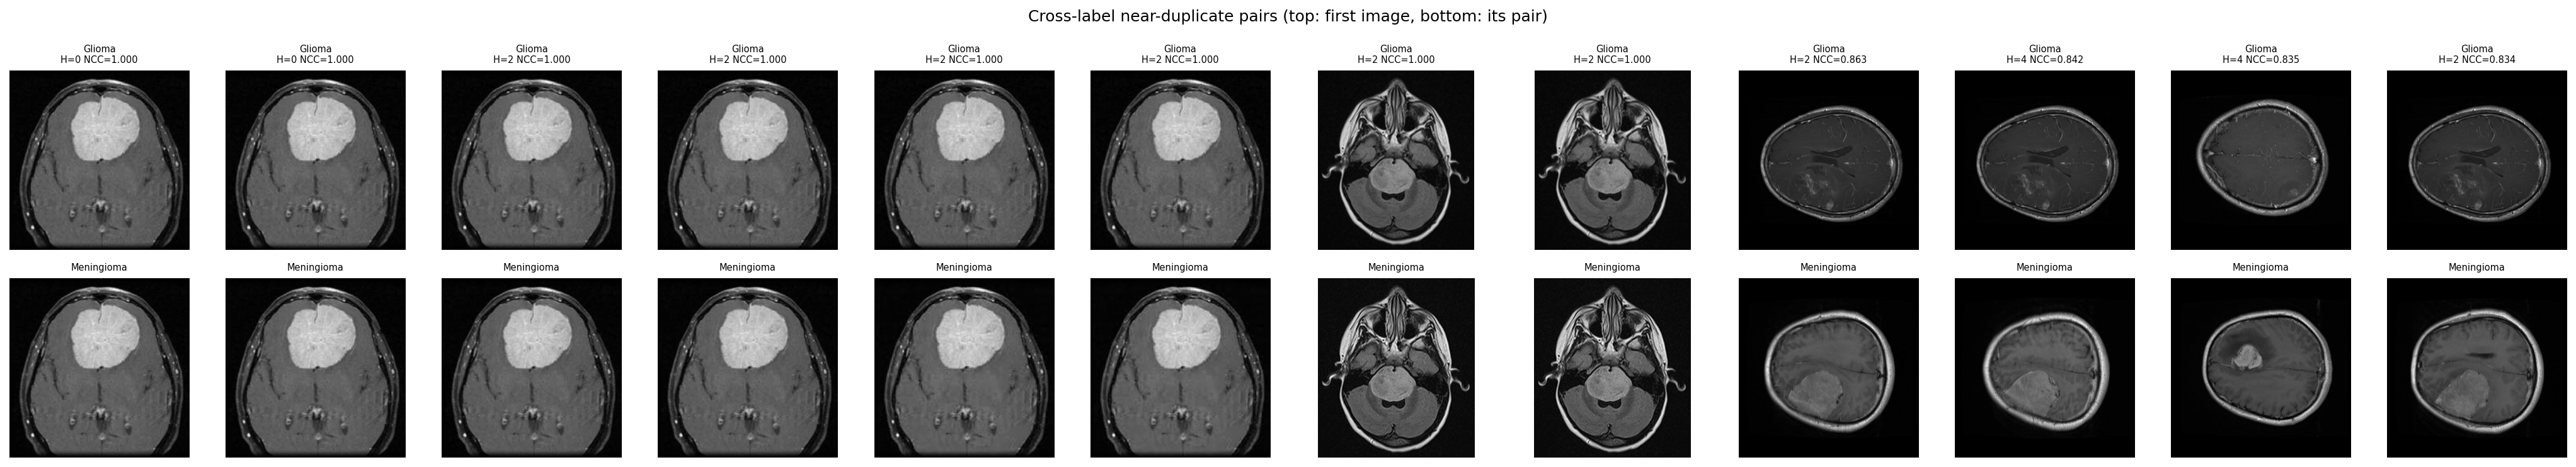
\includegraphics[width=\linewidth]{classification/plots/04_cross_label_pairs.png}
\caption{Multiclass cross-label pairs within Hamming distance 5, label-noise pairs first. All 31 pairs are glioma against meningioma; the 8 pairs at $\mathrm{NCC}\geq 0.98$ lie inside the Bhuvaji collection and both copies were excluded, and the 23 others are hash false positives and were kept. The binary pool has no cross-label pair.}
\end{figure}

\begin{figure}[htbp]
\centering
\panel{1.0}{binary-detection/plots/05_groups_and_leakage.png}{Binary detection: 821 groups, the largest of 7 images.}\\[4pt]
\panel{1.0}{classification/plots/05_groups_and_leakage.png}{Subtype classification: 1,867 groups, the largest of 1,431 images.}
\caption{Group sizes and the distance from each test image to its nearest development image. No test image has a development image within Hamming distance 5 or 8 or at $\mathrm{NCC}\geq 0.98$ (\texttt{leakage\_audit.csv}).}
\end{figure}

\begin{figure}[htbp]
\centering
\panel{1.0}{binary-detection/plots/06_augmentation.png}{Binary detection.}\\[4pt]
\panel{1.0}{classification/plots/06_augmentation.png}{Subtype classification.}
\caption{Training augmentation (horizontal flip, rotation up to $\pm 10^{\circ}$, brightness and contrast jitter of 20\%) on a few training images, with the background-only and head-only inputs of the masking and shortcut tests.}
\end{figure}

\FloatBarrier
\section*{S2. Training}

\begin{figure}[htbp]
\centering
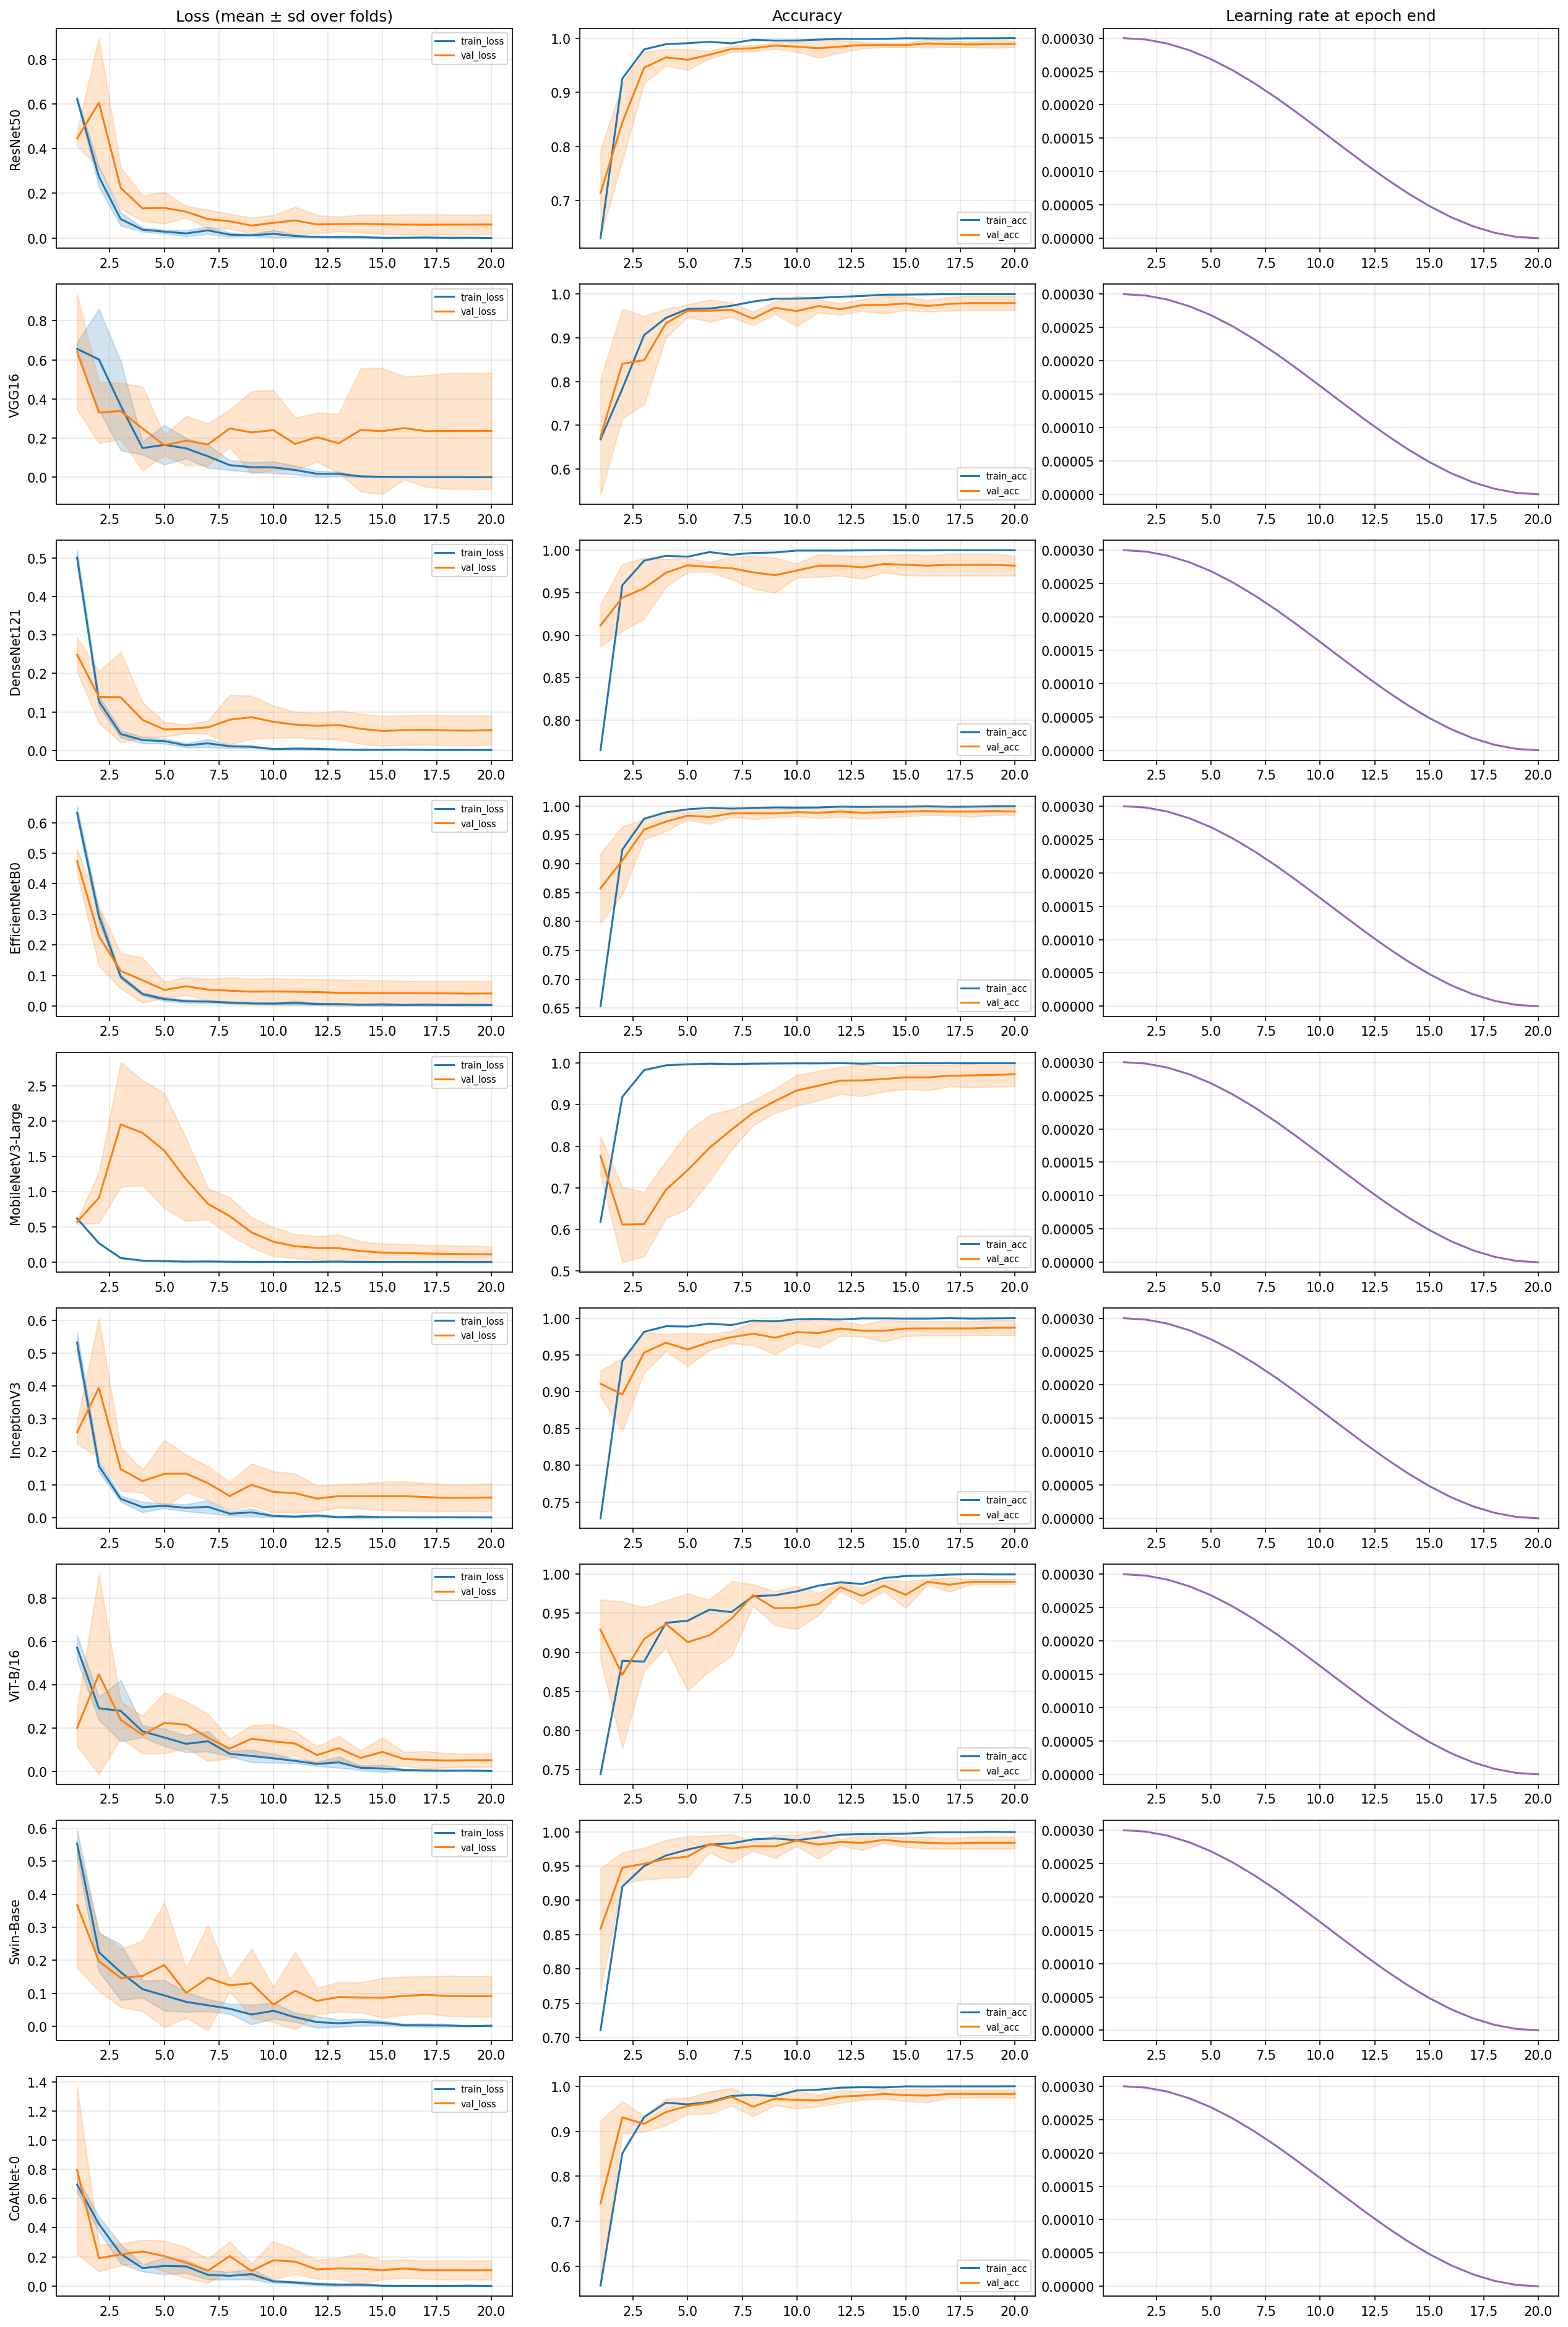
\includegraphics[width=\linewidth]{binary-detection/plots/07_training_curves.png}
\caption{Binary detection: mean $\pm$ one standard deviation across folds of training and validation loss, validation accuracy and learning rate, per model.}
\end{figure}

\begin{figure}[htbp]
\centering
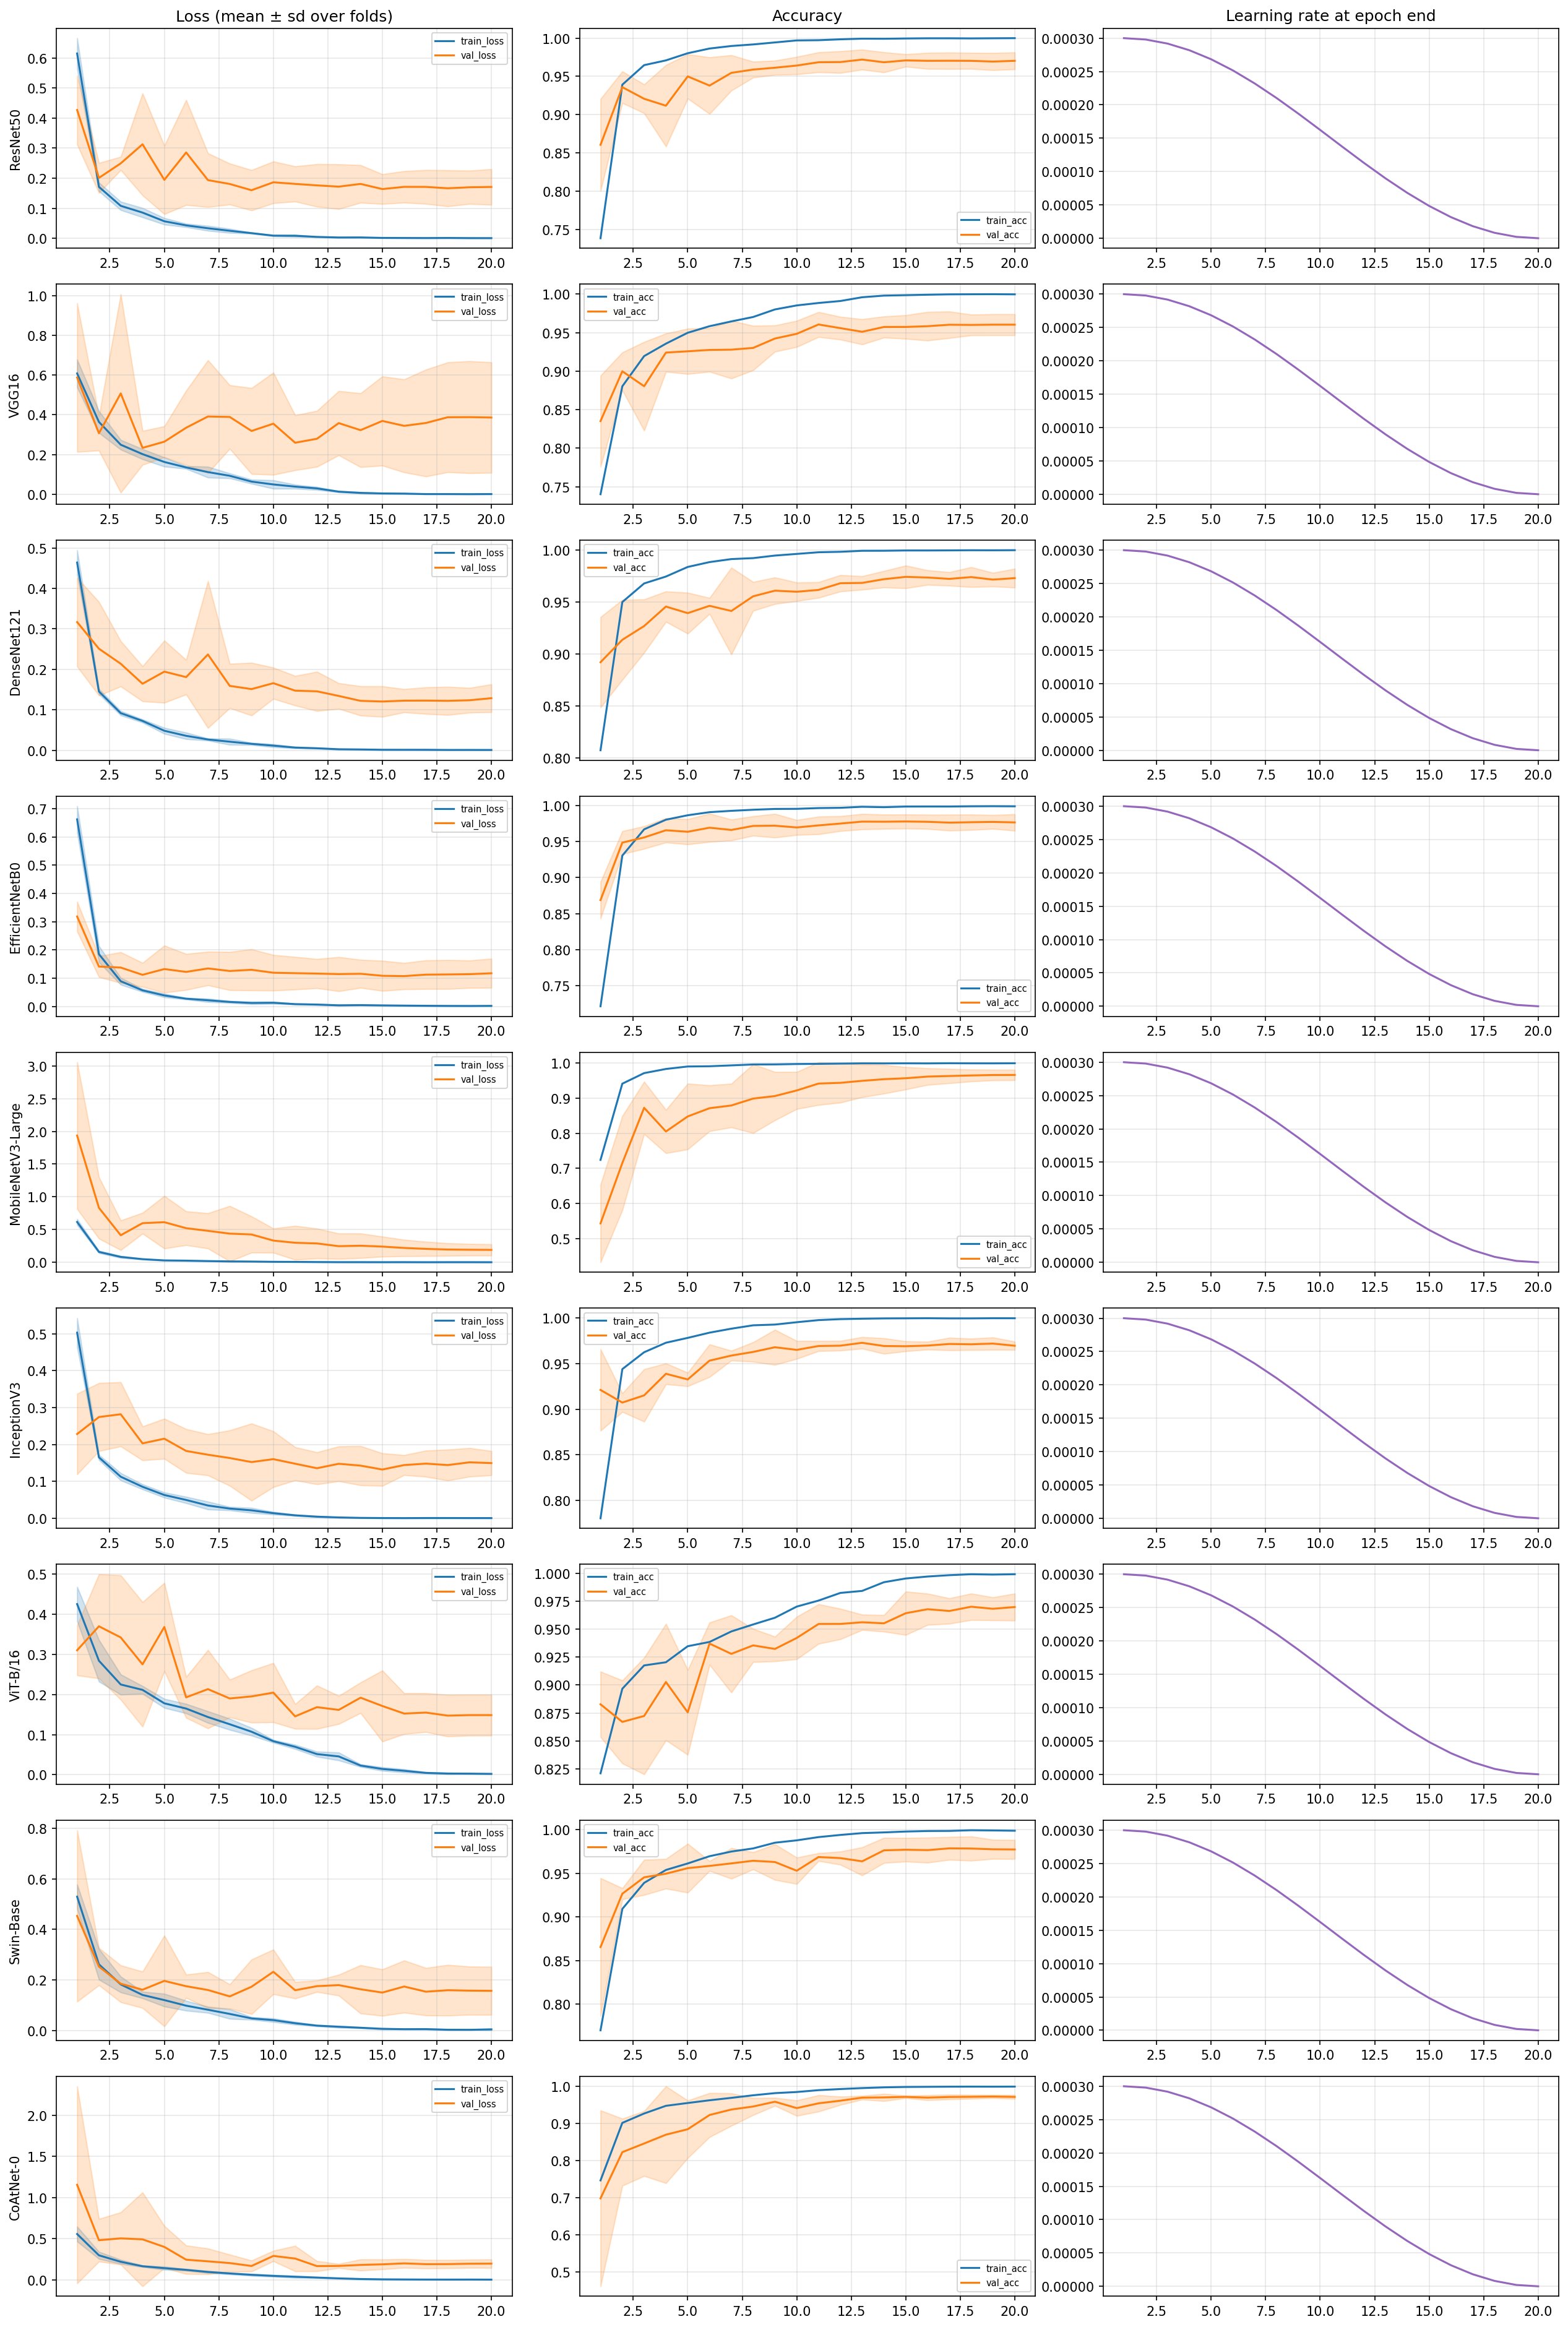
\includegraphics[width=\linewidth]{classification/plots/07_training_curves.png}
\caption{Subtype classification: mean $\pm$ one standard deviation across folds of training and validation loss, validation accuracy and learning rate, per model.}
\end{figure}

\begin{table}[htbp]
\centering
\caption{Binary detection: every full-image run (\texttt{run\_metrics.csv}). Every run took 260 optimiser steps. $T$ is the temperature fitted on the run's validation fold and Thr.\ the Youden threshold chosen there; accuracy and log-loss are on the 171 test images after temperature scaling. In fold 4 the temperature of six models lies at or near the lower search bound $e^{-3}\approx 0.0498$.}
\scriptsize
\begin{tabular*}{\textwidth}{@{\extracolsep{\fill}}lccccccc@{}}
\toprule
Model & Fold & Best epoch & $T$ & Thr. & Test accuracy & Test log-loss & Train images \\
\midrule
\multirow{5}{*}{CoAtNet-0} & 0 & 9 & 1.1767 & 0.739 & 0.9883 & 0.0491 & 830 \\
 & 1 & 7 & 1.4761 & 0.529 & 0.9825 & 0.0534 & 803 \\
 & 2 & 12 & 1.7756 & 0.633 & 0.9474 & 0.1317 & 807 \\
 & 3 & 14 & 2.1222 & 0.316 & 0.9883 & 0.0333 & 804 \\
 & 4 & 7 & 0.0604 & 1.000 & 0.9708 & 0.8079 & 812 \\
\midrule
\multirow{5}{*}{DenseNet121} & 0 & 6 & 0.8003 & 0.724 & 0.9766 & 0.0847 & 830 \\
 & 1 & 11 & 1.0106 & 0.657 & 0.9649 & 0.0751 & 803 \\
 & 2 & 12 & 1.3466 & 0.885 & 0.9649 & 0.1019 & 807 \\
 & 3 & 14 & 1.1351 & 0.950 & 0.9825 & 0.0696 & 804 \\
 & 4 & 15 & 0.5882 & 0.927 & 0.9708 & 0.2513 & 812 \\
\midrule
\multirow{5}{*}{EfficientNetB0} & 0 & 5 & 1.2527 & 0.621 & 0.9708 & 0.0875 & 830 \\
 & 1 & 14 & 1.2311 & 0.962 & 0.9766 & 0.0378 & 803 \\
 & 2 & 13 & 1.1739 & 0.625 & 0.9825 & 0.0471 & 807 \\
 & 3 & 11 & 0.9215 & 0.985 & 0.9825 & 0.0755 & 804 \\
 & 4 & 19 & 0.0498 & 1.000 & 0.9766 & 0.5431 & 812 \\
\midrule
\multirow{5}{*}{InceptionV3} & 0 & 17 & 1.6119 & 0.895 & 0.9766 & 0.0543 & 830 \\
 & 1 & 8 & 1.4656 & 0.045 & 0.9766 & 0.0603 & 803 \\
 & 2 & 10 & 0.9470 & 0.861 & 0.9766 & 0.1005 & 807 \\
 & 3 & 5 & 1.1069 & 0.829 & 0.9825 & 0.0372 & 804 \\
 & 4 & 12 & 0.0682 & 1.000 & 0.9825 & 0.3662 & 812 \\
\midrule
\multirow{5}{*}{MobileNetV3-Large} & 0 & 20 & 2.7638 & 0.121 & 0.9298 & 0.1551 & 830 \\
 & 1 & 20 & 1.8160 & 0.583 & 0.9766 & 0.0638 & 803 \\
 & 2 & 14 & 1.6694 & 0.410 & 0.9883 & 0.0448 & 807 \\
 & 3 & 20 & 1.7832 & 0.249 & 0.9591 & 0.1161 & 804 \\
 & 4 & 13 & 0.0508 & 1.000 & 0.9649 & 0.7224 & 812 \\
\midrule
\multirow{5}{*}{ResNet50} & 0 & 9 & 1.7422 & 0.819 & 0.9474 & 0.1451 & 830 \\
 & 1 & 8 & 1.7905 & 0.314 & 0.9766 & 0.0837 & 803 \\
 & 2 & 7 & 1.0362 & 0.853 & 0.9649 & 0.0787 & 807 \\
 & 3 & 17 & 1.2096 & 0.759 & 0.9708 & 0.1416 & 804 \\
 & 4 & 12 & 0.0498 & 1.000 & 0.9825 & 0.4848 & 812 \\
\midrule
\multirow{5}{*}{Swin-Base} & 0 & 14 & 1.7903 & 0.617 & 0.9708 & 0.0826 & 830 \\
 & 1 & 11 & 1.7026 & 0.550 & 0.9708 & 0.1311 & 803 \\
 & 2 & 6 & 1.5159 & 0.683 & 0.9591 & 0.1221 & 807 \\
 & 3 & 5 & 0.8935 & 0.261 & 0.9883 & 0.0536 & 804 \\
 & 4 & 10 & 0.0498 & 1.000 & 1.0000 & 0.0000 & 812 \\
\midrule
\multirow{5}{*}{VGG16} & 0 & 5 & 1.7926 & 0.462 & 0.9532 & 0.1252 & 830 \\
 & 1 & 13 & 2.1367 & 0.216 & 0.9649 & 0.0912 & 803 \\
 & 2 & 18 & 1.5436 & 0.775 & 0.9649 & 0.2265 & 807 \\
 & 3 & 4 & 1.4973 & 0.196 & 0.9474 & 0.1276 & 804 \\
 & 4 & 6 & 1.8620 & 0.495 & 0.9649 & 0.1407 & 812 \\
\midrule
\multirow{5}{*}{ViT-B/16} & 0 & 17 & 1.4451 & 0.767 & 0.9825 & 0.0566 & 830 \\
 & 1 & 12 & 1.5874 & 0.483 & 0.9649 & 0.1114 & 803 \\
 & 2 & 17 & 1.3066 & 0.824 & 0.9883 & 0.0526 & 807 \\
 & 3 & 8 & 0.8068 & 0.559 & 0.9708 & 0.0711 & 804 \\
 & 4 & 16 & 0.9993 & 0.836 & 0.9708 & 0.1007 & 812 \\
\bottomrule
\end{tabular*}
\end{table}

\begin{table}[htbp]
\centering
\caption{Subtype classification: every full-image run (\texttt{run\_metrics.csv}). Optimiser steps depend on the fold because the group-aware folds differ in size; within a fold they are equal for every model. In fold 0, whose validation fold has 154 images, the temperature of EfficientNetB0, InceptionV3 and Swin-Base lies at or near the lower search bound.}
\scriptsize
\begin{tabular*}{\textwidth}{@{\extracolsep{\fill}}lccccccc@{}}
\toprule
Model & Fold & Steps & Best epoch & $T$ & Test accuracy & Test log-loss & Train / val images \\
\midrule
\multirow{5}{*}{CoAtNet-0} & 0 & 1,420 & 7 & 0.8899 & 1.0000 & 0.0209 & 4,531 / 154 \\
 & 1 & 1,240 & 9 & 1.3042 & 1.0000 & 0.0034 & 3,943 / 742 \\
 & 2 & 1,260 & 5 & 0.8503 & 0.9778 & 0.0720 & 3,988 / 697 \\
 & 3 & 1,200 & 6 & 1.2193 & 0.9778 & 0.0395 & 3,809 / 876 \\
 & 4 & 780 & 15 & 2.3073 & 0.9778 & 0.0236 & 2,469 / 2,216 \\
\midrule
\multirow{5}{*}{DenseNet121} & 0 & 1,420 & 7 & 1.1754 & 1.0000 & 0.0040 & 4,531 / 154 \\
 & 1 & 1,240 & 15 & 1.9404 & 1.0000 & 0.0061 & 3,943 / 742 \\
 & 2 & 1,260 & 9 & 1.5745 & 1.0000 & 0.0186 & 3,988 / 697 \\
 & 3 & 1,200 & 4 & 1.4594 & 0.9778 & 0.1067 & 3,809 / 876 \\
 & 4 & 780 & 10 & 1.5314 & 0.9778 & 0.0355 & 2,469 / 2,216 \\
\midrule
\multirow{5}{*}{EfficientNetB0} & 0 & 1,420 & 9 & 0.0498 & 0.9778 & 0.6140 & 4,531 / 154 \\
 & 1 & 1,240 & 4 & 1.5348 & 0.9111 & 0.1585 & 3,943 / 742 \\
 & 2 & 1,260 & 15 & 1.8186 & 1.0000 & 0.0024 & 3,988 / 697 \\
 & 3 & 1,200 & 3 & 1.3621 & 1.0000 & 0.0181 & 3,809 / 876 \\
 & 4 & 780 & 16 & 1.7429 & 0.9778 & 0.0330 & 2,469 / 2,216 \\
\midrule
\multirow{5}{*}{InceptionV3} & 0 & 1,420 & 9 & 0.0515 & 1.0000 & 0.0000 & 4,531 / 154 \\
 & 1 & 1,240 & 7 & 1.5646 & 1.0000 & 0.0050 & 3,943 / 742 \\
 & 2 & 1,260 & 10 & 1.6805 & 1.0000 & 0.0040 & 3,988 / 697 \\
 & 3 & 1,200 & 15 & 2.2675 & 1.0000 & 0.0101 & 3,809 / 876 \\
 & 4 & 780 & 11 & 1.7383 & 0.9778 & 0.0503 & 2,469 / 2,216 \\
\midrule
\multirow{5}{*}{MobileNetV3-Large} & 0 & 1,420 & 12 & 1.0519 & 0.9778 & 0.1369 & 4,531 / 154 \\
 & 1 & 1,240 & 20 & 3.1578 & 0.9778 & 0.0712 & 3,943 / 742 \\
 & 2 & 1,260 & 18 & 2.6818 & 0.9778 & 0.0685 & 3,988 / 697 \\
 & 3 & 1,200 & 8 & 2.4891 & 0.9778 & 0.0327 & 3,809 / 876 \\
 & 4 & 780 & 20 & 3.0036 & 0.9778 & 0.0689 & 2,469 / 2,216 \\
\midrule
\multirow{5}{*}{ResNet50} & 0 & 1,420 & 5 & 0.9164 & 1.0000 & 0.0026 & 4,531 / 154 \\
 & 1 & 1,240 & 9 & 2.0543 & 0.9778 & 0.0395 & 3,943 / 742 \\
 & 2 & 1,260 & 5 & 1.5465 & 0.9778 & 0.0672 & 3,988 / 697 \\
 & 3 & 1,200 & 15 & 2.6184 & 1.0000 & 0.0176 & 3,809 / 876 \\
 & 4 & 780 & 8 & 1.6629 & 0.9778 & 0.0957 & 2,469 / 2,216 \\
\midrule
\multirow{5}{*}{Swin-Base} & 0 & 1,420 & 15 & 0.0498 & 1.0000 & 0.0000 & 4,531 / 154 \\
 & 1 & 1,240 & 8 & 1.6375 & 1.0000 & 0.0112 & 3,943 / 742 \\
 & 2 & 1,260 & 9 & 1.9777 & 1.0000 & 0.0076 & 3,988 / 697 \\
 & 3 & 1,200 & 5 & 1.7771 & 0.9778 & 0.0397 & 3,809 / 876 \\
 & 4 & 780 & 18 & 2.2403 & 1.0000 & 0.0047 & 2,469 / 2,216 \\
\midrule
\multirow{5}{*}{VGG16} & 0 & 1,420 & 11 & 1.2077 & 0.9778 & 0.1367 & 4,531 / 154 \\
 & 1 & 1,240 & 7 & 1.7136 & 1.0000 & 0.0175 & 3,943 / 742 \\
 & 2 & 1,260 & 2 & 1.6416 & 0.9333 & 0.2497 & 3,988 / 697 \\
 & 3 & 1,200 & 4 & 2.0744 & 0.9778 & 0.0520 & 3,809 / 876 \\
 & 4 & 780 & 13 & 2.2774 & 0.9778 & 0.0970 & 2,469 / 2,216 \\
\midrule
\multirow{5}{*}{ViT-B/16} & 0 & 1,420 & 15 & 1.3910 & 1.0000 & 0.0020 & 4,531 / 154 \\
 & 1 & 1,240 & 13 & 1.7649 & 1.0000 & 0.0238 & 3,943 / 742 \\
 & 2 & 1,260 & 13 & 1.2801 & 0.9778 & 0.0420 & 3,988 / 697 \\
 & 3 & 1,200 & 11 & 1.5805 & 1.0000 & 0.0129 & 3,809 / 876 \\
 & 4 & 780 & 11 & 1.4512 & 0.9778 & 0.1176 & 2,469 / 2,216 \\
\bottomrule
\end{tabular*}
\end{table}

\FloatBarrier
\section*{S3. Test results}

\begin{table}[htbp]
\centering
\caption{Per-class test metrics of the fold ensembles (\texttt{test\_per\_class.csv}). Binary support: 64 tumour-negative, 107 tumour. Multiclass support: 1 glioma, 13 meningioma, 31 pituitary.}
\scriptsize
\begin{tabular*}{\textwidth}{@{\extracolsep{\fill}}llcccccc@{}}
\toprule
Model & Class & TP & FP & FN & Precision & Sensitivity & Specificity \\
\midrule
\multirow{2}{*}{ResNet50} & Tumour-negative & 63 & 2 & 1 & 0.9692 & 0.9844 & 0.9813 \\
 & Tumour & 105 & 1 & 2 & 0.9906 & 0.9813 & 0.9844 \\
\multirow{2}{*}{VGG16} & Tumour-negative & 62 & 3 & 2 & 0.9538 & 0.9688 & 0.9720 \\
 & Tumour & 104 & 2 & 3 & 0.9811 & 0.9720 & 0.9688 \\
\multirow{2}{*}{DenseNet121} & Tumour-negative & 60 & 1 & 4 & 0.9836 & 0.9375 & 0.9907 \\
 & Tumour & 106 & 4 & 1 & 0.9636 & 0.9907 & 0.9375 \\
\multirow{2}{*}{EfficientNetB0} & Tumour-negative & 63 & 0 & 1 & 1.0000 & 0.9844 & 1.0000 \\
 & Tumour & 107 & 1 & 0 & 0.9907 & 1.0000 & 0.9844 \\
\multirow{2}{*}{MobileNetV3-Large} & Tumour-negative & 62 & 3 & 2 & 0.9538 & 0.9688 & 0.9720 \\
 & Tumour & 104 & 2 & 3 & 0.9811 & 0.9720 & 0.9688 \\
\multirow{2}{*}{InceptionV3} & Tumour-negative & 62 & 1 & 2 & 0.9841 & 0.9688 & 0.9907 \\
 & Tumour & 106 & 2 & 1 & 0.9815 & 0.9907 & 0.9688 \\
\multirow{2}{*}{ViT-B/16} & Tumour-negative & 63 & 0 & 1 & 1.0000 & 0.9844 & 1.0000 \\
 & Tumour & 107 & 1 & 0 & 0.9907 & 1.0000 & 0.9844 \\
\multirow{2}{*}{Swin-Base} & Tumour-negative & 64 & 2 & 0 & 0.9697 & 1.0000 & 0.9813 \\
 & Tumour & 105 & 0 & 2 & 1.0000 & 0.9813 & 1.0000 \\
\multirow{2}{*}{CoAtNet-0} & Tumour-negative & 64 & 1 & 0 & 0.9846 & 1.0000 & 0.9907 \\
 & Tumour & 106 & 0 & 1 & 1.0000 & 0.9907 & 1.0000 \\
\midrule
\multirow{3}{*}{\shortstack[l]{ResNet50, DenseNet121, InceptionV3,\\ViT-B/16, Swin-Base, CoAtNet-0}} & Glioma & 1 & 0 & 0 & 1.0000 & 1.0000 & 1.0000 \\
 & Meningioma & 13 & 0 & 0 & 1.0000 & 1.0000 & 1.0000 \\
 & Pituitary & 31 & 0 & 0 & 1.0000 & 1.0000 & 1.0000 \\
\midrule
\multirow{3}{*}{\shortstack[l]{VGG16, EfficientNetB0,\\MobileNetV3-Large}} & Glioma & 1 & 1 & 0 & 0.5000 & 1.0000 & 0.9773 \\
 & Meningioma & 12 & 0 & 1 & 1.0000 & 0.9231 & 1.0000 \\
 & Pituitary & 31 & 0 & 0 & 1.0000 & 1.0000 & 1.0000 \\
\bottomrule
\end{tabular*}
\end{table}

\begin{table}[htbp]
\centering
\caption{Fold-ensemble test accuracy by the Hamming distance from each test image to its nearest development image (\texttt{accuracy\_by\_nearest\_dev\_distance.csv}). The multiclass test set has no image at distance 17 to 20.}
\small
\begin{tabular*}{\textwidth}{@{\extracolsep{\fill}}lccccc@{}}
\toprule
 & \multicolumn{3}{c}{Binary detection} & \multicolumn{2}{c}{Subtype classification} \\
\cmidrule(lr){2-4}\cmidrule(l){5-6}
Model & 9--12 & 13--16 & 17--20 & 9--12 & 13--16 \\
\midrule
CoAtNet-0 & 0.9886 & 1.0000 & 1.0000 & 1.0000 & 1.0000 \\
DenseNet121 & 0.9773 & 0.9589 & 1.0000 & 1.0000 & 1.0000 \\
EfficientNetB0 & 1.0000 & 0.9863 & 1.0000 & 0.9773 & 1.0000 \\
InceptionV3 & 1.0000 & 0.9589 & 1.0000 & 1.0000 & 1.0000 \\
MobileNetV3-Large & 0.9545 & 0.9863 & 1.0000 & 0.9773 & 1.0000 \\
ResNet50 & 0.9886 & 0.9726 & 1.0000 & 1.0000 & 1.0000 \\
Swin-Base & 1.0000 & 0.9726 & 1.0000 & 1.0000 & 1.0000 \\
VGG16 & 0.9659 & 0.9726 & 1.0000 & 0.9773 & 1.0000 \\
ViT-B/16 & 1.0000 & 0.9863 & 1.0000 & 1.0000 & 1.0000 \\
\bottomrule
\end{tabular*}
\end{table}

\begin{figure}[htbp]
\centering
\panel{1.0}{binary-detection/plots/10_roc_pr_curves.png}{Binary detection, tumour class.}\\[4pt]
\panel{1.0}{classification/plots/10_roc_pr_curves.png}{Subtype classification, one-versus-rest.}
\caption{Receiver operating characteristic and precision--recall curves of every fold ensemble on the test set.}
\end{figure}

\begin{figure}[htbp]
\centering
\panel{0.49}{binary-detection/plots/08_mcnemar.png}{Binary detection.}\hfill
\panel{0.49}{classification/plots/08_mcnemar.png}{Subtype classification.}
\caption{Holm-corrected exact McNemar p-values between the fold ensembles. Every adjusted p-value is 1.0 in both tasks (\texttt{mcnemar\_holm\_p.csv}).}
\end{figure}

\begin{figure}[htbp]
\centering
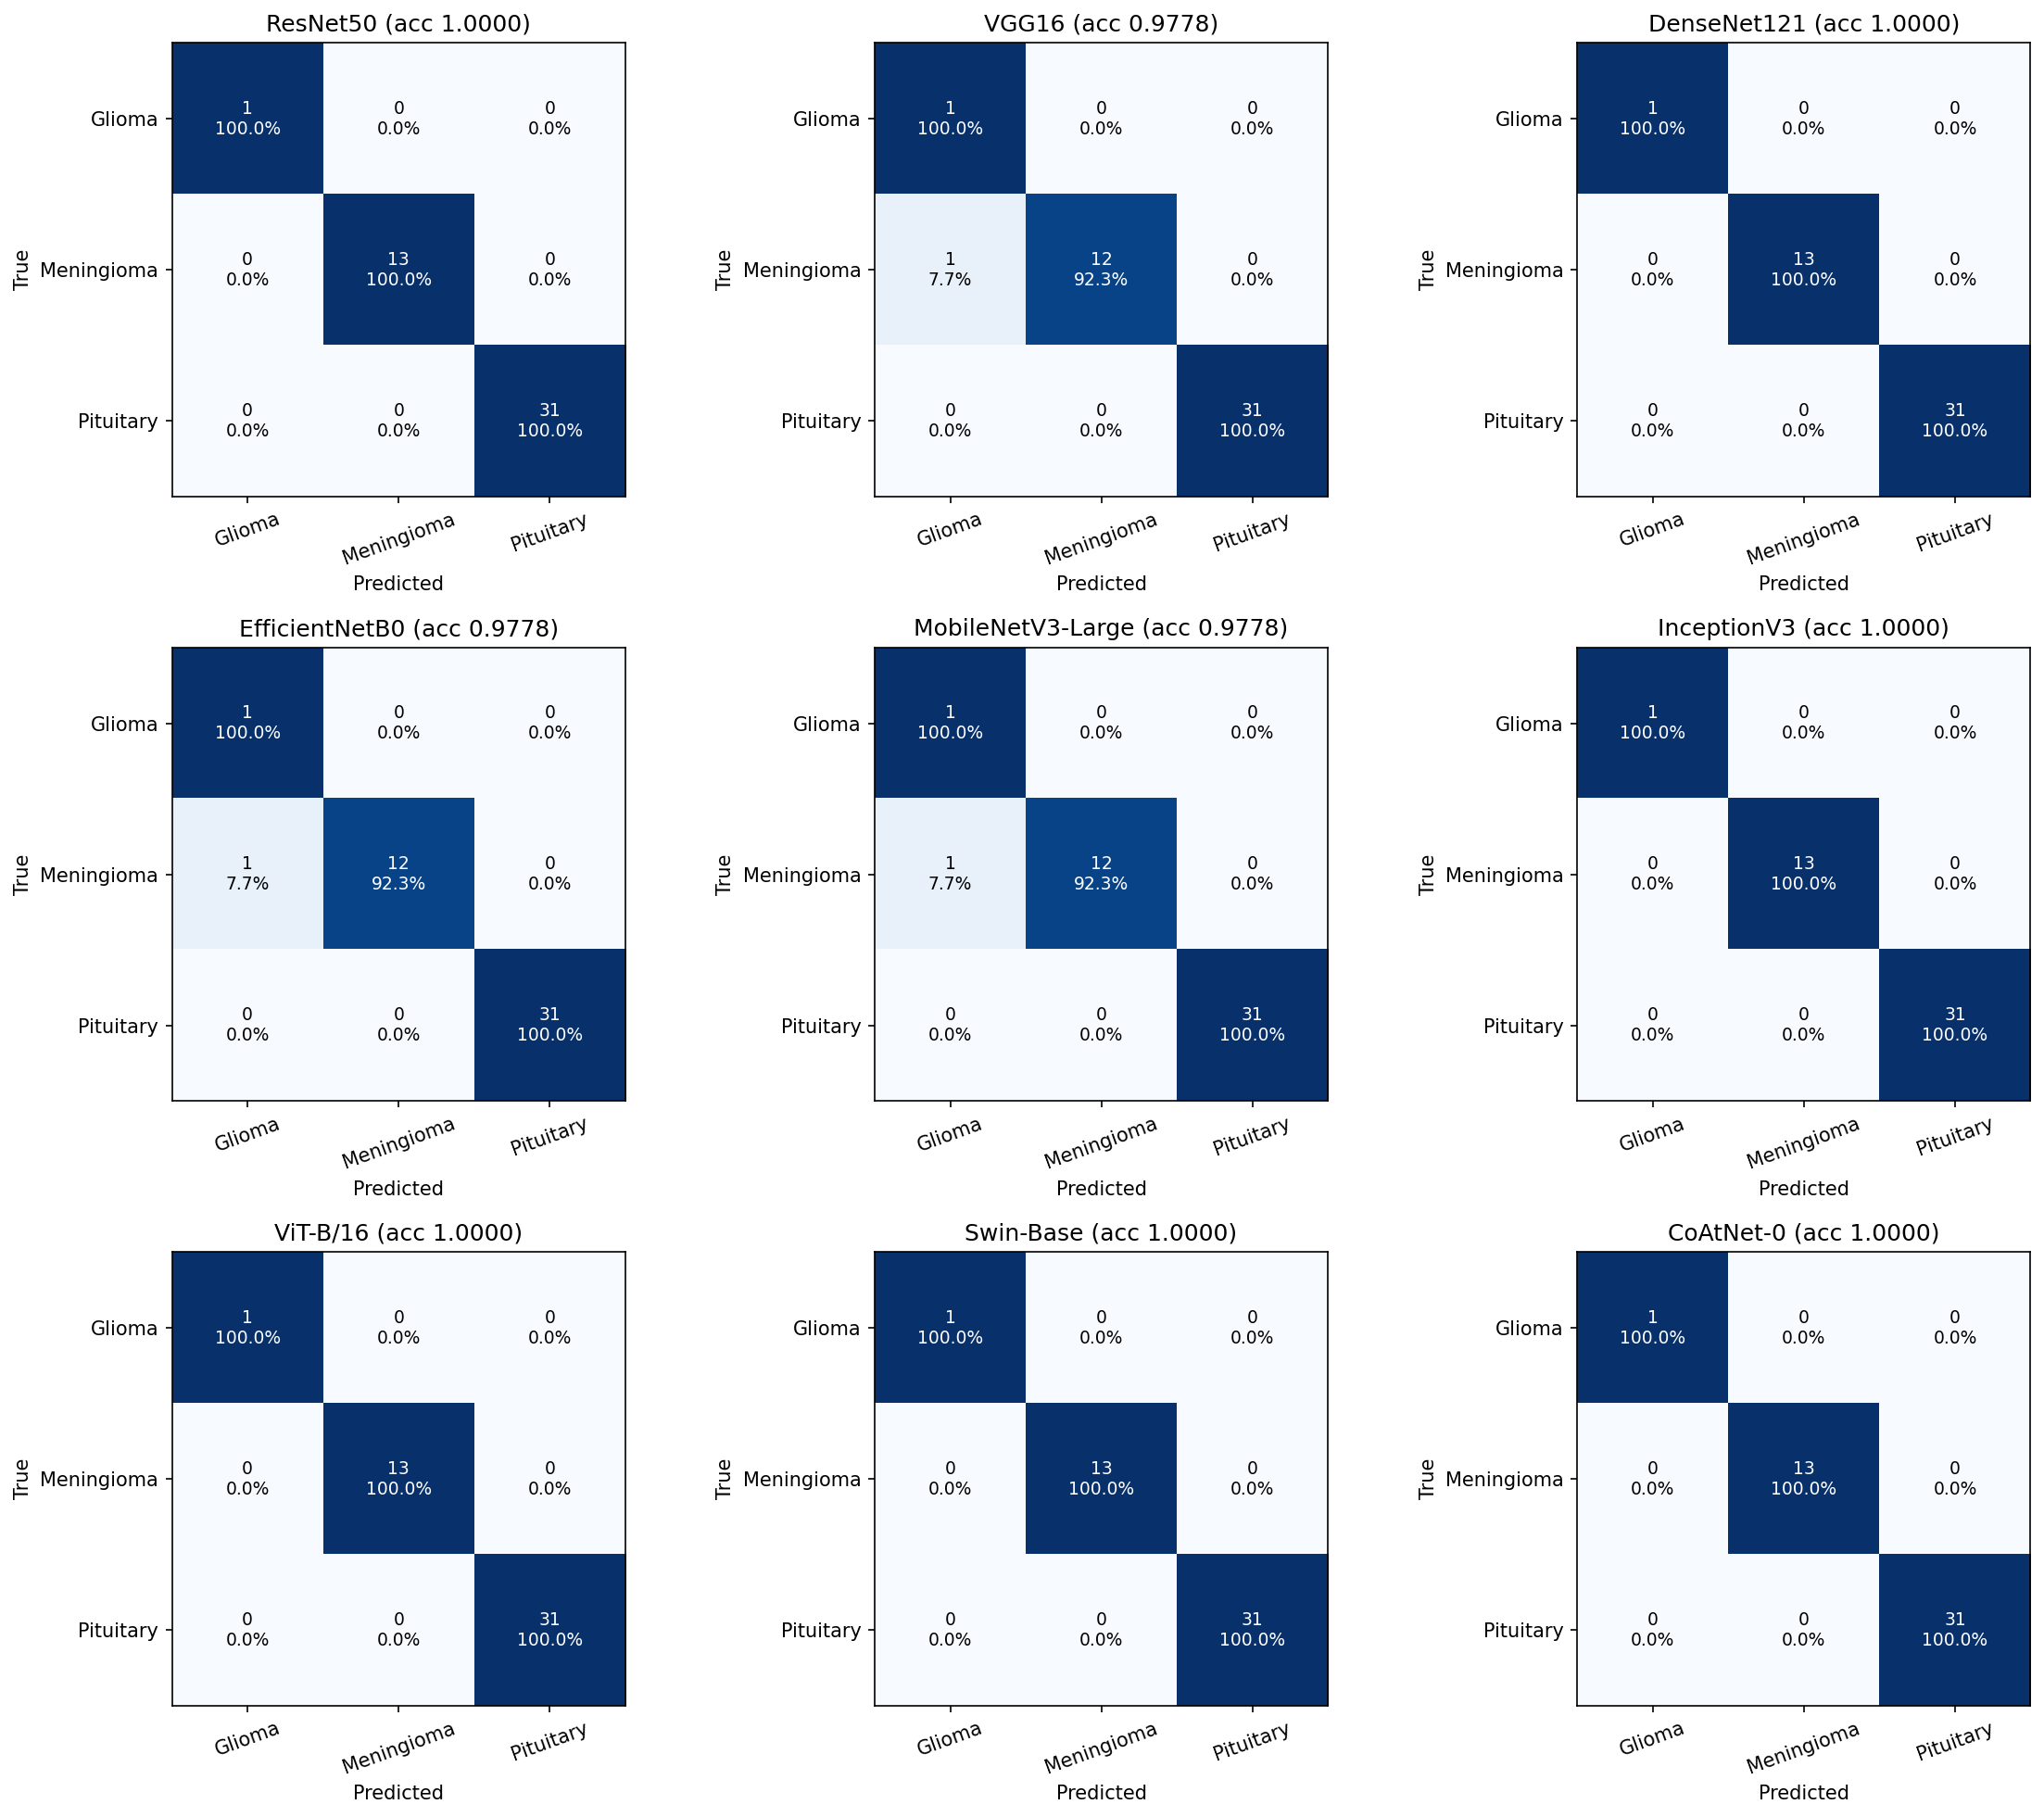
\includegraphics[width=\linewidth]{classification/plots/09_confusion_matrices.png}
\caption{Subtype classification: test confusion matrices of every fold ensemble, counts with row percentages.}
\end{figure}

\begin{figure}[htbp]
\centering
\panel{1.0}{binary-detection/plots/11_calibration.png}{Binary detection.}\\[4pt]
\panel{1.0}{classification/plots/11_calibration.png}{Subtype classification.}
\caption{Reliability diagrams of every fold ensemble on the test set, uncalibrated and temperature-scaled, with the expected calibration error of each.}
\end{figure}

\begin{figure}[htbp]
\centering
\panel{0.49}{binary-detection/plots/12_accuracy_by_distance.png}{Binary detection.}\hfill
\panel{0.49}{classification/plots/12_accuracy_by_distance.png}{Subtype classification.}
\caption{Test accuracy by the Hamming distance from each test image to its nearest development image.}
\end{figure}

\FloatBarrier
\section*{S4. Efficiency}

\begin{table}[htbp]
\centering
\caption{Complete efficiency measurements (\texttt{efficiency.csv}): latency (ms) and throughput at batch size 32 (images/s) as mean $\pm$ pooled standard deviation over three repeats on one Tesla T4 under half-precision autocasting; training throughput (images/s) and peak training memory (GB) averaged over the folds. Training throughput is a lower bound because the two workers shared four CPU cores.}
\scriptsize
\begin{tabular*}{\textwidth}{@{\extracolsep{\fill}}llcccc@{}}
\toprule
Task & Model & Latency (ms) & Throughput (img/s) & Training (img/s) & Peak memory (GB) \\
\midrule
\multirow{9}{*}{Binary} & ResNet50 & $9.57\pm 0.38$ & $777.2\pm 6.1$ & 235.2 & 5.62 \\
 & VGG16 & $7.72\pm 0.42$ & $386.5\pm 4.8$ & 124.4 & 9.88 \\
 & DenseNet121 & $23.58\pm 1.53$ & $656.6\pm 22.9$ & 185.4 & 4.48 \\
 & EfficientNetB0 & $13.13\pm 0.55$ & $1393.3\pm 115.8$ & 136.4 & 3.09 \\
 & MobileNetV3-Large & $10.55\pm 1.09$ & $2301.1\pm 292.9$ & 182.3 & 2.09 \\
 & InceptionV3 & $17.63\pm 0.79$ & $511.6\pm 5.8$ & 155.8 & 5.85 \\
 & ViT-B/16 & $10.95\pm 1.04$ & $272.2\pm 2.8$ & 93.0 & 5.96 \\
 & Swin-Base & $36.29\pm 1.23$ & $197.6\pm 2.9$ & 62.9 & 6.45 \\
 & CoAtNet-0 & $16.53\pm 1.07$ & $513.1\pm 6.9$ & 118.7 & 11.39 \\
\midrule
\multirow{9}{*}{Multiclass} & ResNet50 & $9.07\pm 0.36$ & $716.8\pm 6.9$ & 232.9 & 4.08 \\
 & VGG16 & $8.02\pm 0.40$ & $332.1\pm 6.2$ & 130.5 & 9.87 \\
 & DenseNet121 & $22.81\pm 1.22$ & $607.7\pm 17.7$ & 180.4 & 4.48 \\
 & EfficientNetB0 & $12.81\pm 0.80$ & $1265.7\pm 50.3$ & 243.9 & 3.04 \\
 & MobileNetV3-Large & $9.99\pm 0.92$ & $2183.1\pm 234.4$ & 355.2 & 2.08 \\
 & InceptionV3 & $16.69\pm 1.25$ & $438.2\pm 6.6$ & 155.4 & 5.26 \\
 & ViT-B/16 & $10.26\pm 1.10$ & $241.0\pm 3.0$ & 82.6 & 5.97 \\
 & Swin-Base & $34.65\pm 1.51$ & $173.1\pm 2.8$ & 57.8 & 6.45 \\
 & CoAtNet-0 & $15.88\pm 0.73$ & $448.4\pm 6.3$ & 131.1 & 10.42 \\
\bottomrule
\end{tabular*}
\end{table}

\begin{figure}[htbp]
\centering
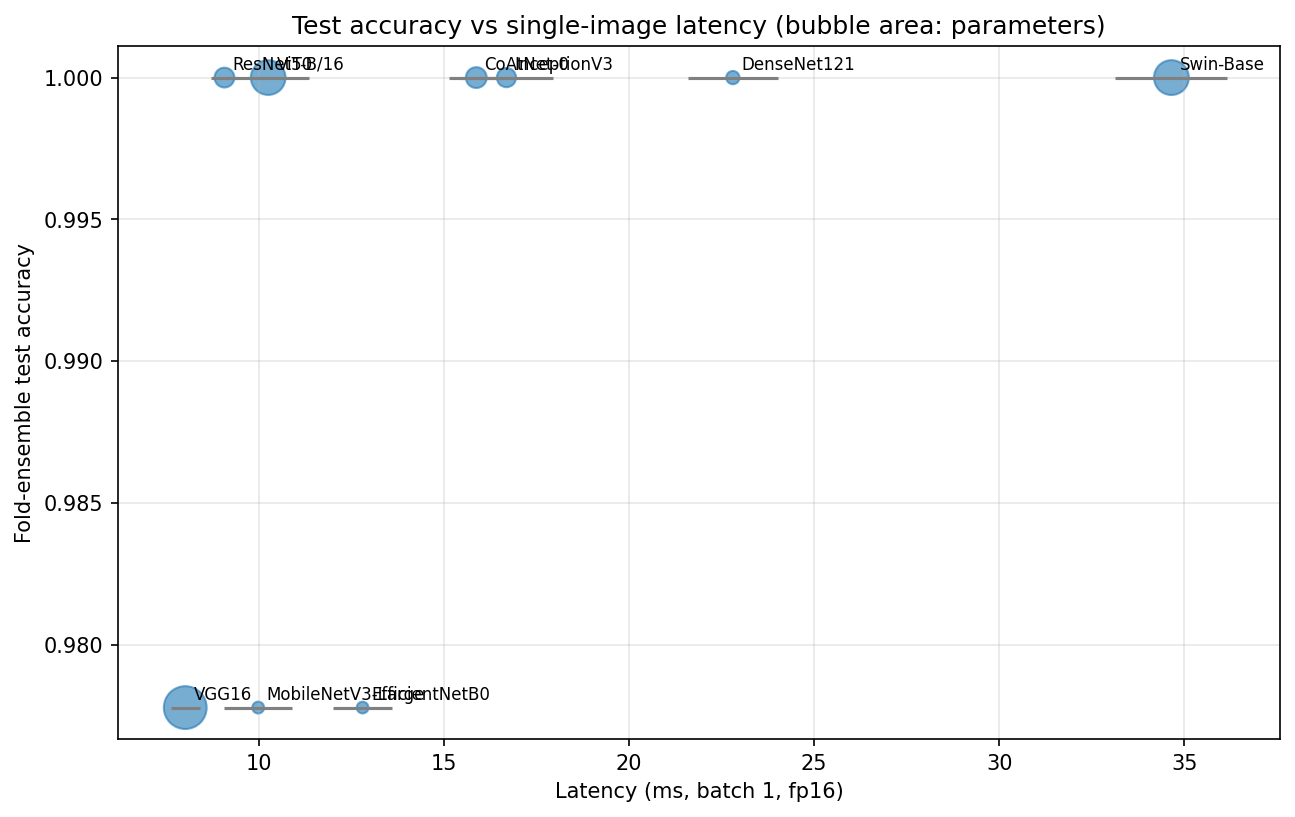
\includegraphics[width=0.85\linewidth]{classification/plots/18_accuracy_vs_latency.png}
\caption{Subtype classification: fold-ensemble test accuracy against single-image latency for every model.}
\end{figure}

\FloatBarrier
\section*{S5. Attention and shortcut analysis}

\begin{table}[htbp]
\centering
\caption{Share of Grad-CAM energy outside the head mask, mean $\pm$ standard deviation over test images (\texttt{outside\_head\_energy.csv}), and of occlusion sensitivity over 16 binary and 17 multiclass test images (\texttt{occlusion\_outside\_head.csv}). The multiclass test set has one glioma image, so that column has no standard deviation.}
\scriptsize
\setlength{\tabcolsep}{3pt}
\begin{tabular*}{\textwidth}{@{\extracolsep{\fill}}lcccccccc@{}}
\toprule
 & \multicolumn{3}{c}{Binary detection} & \multicolumn{4}{c}{Subtype classification} \\
\cmidrule(lr){2-4}\cmidrule(l){5-8}
Model & Tumour-negative & Tumour & Occlusion & Glioma & Meningioma & Pituitary & Occlusion \\
\midrule
ResNet50 & $0.122\pm 0.219$ & $0.079\pm 0.200$ & 0.116 & 0.098 & $0.056\pm 0.074$ & $0.106\pm 0.202$ & 0.079 \\
VGG16 & $0.153\pm 0.212$ & $0.074\pm 0.184$ & 0.007 & 0.026 & $0.121\pm 0.066$ & $0.115\pm 0.163$ & 0.079 \\
DenseNet121 & $0.190\pm 0.229$ & $0.176\pm 0.183$ & 0.135 & 0.108 & $0.148\pm 0.042$ & $0.150\pm 0.153$ & 0.110 \\
EfficientNetB0 & $0.287\pm 0.211$ & $0.072\pm 0.180$ & 0.194 & 0.033 & $0.067\pm 0.042$ & $0.091\pm 0.156$ & 0.066 \\
MobileNetV3-Large & $0.142\pm 0.231$ & $0.082\pm 0.163$ & 0.111 & 0.038 & $0.058\pm 0.056$ & $0.134\pm 0.136$ & 0.071 \\
InceptionV3 & $0.146\pm 0.234$ & $0.147\pm 0.187$ & 0.167 & 0.102 & $0.136\pm 0.062$ & $0.129\pm 0.178$ & 0.099 \\
ViT-B/16 (Grad-CAM) & $0.426\pm 0.238$ & $0.244\pm 0.264$ & 0.155 & 0.326 & $0.077\pm 0.045$ & $0.218\pm 0.229$ & 0.107 \\
ViT-B/16 (rollout) & $0.421\pm 0.179$ & $0.285\pm 0.163$ & & 0.262 & $0.350\pm 0.047$ & $0.358\pm 0.121$ & \\
Swin-Base & $0.159\pm 0.246$ & $0.185\pm 0.195$ & 0.182 & 0.079 & $0.123\pm 0.046$ & $0.103\pm 0.158$ & 0.122 \\
CoAtNet-0 & $0.139\pm 0.248$ & $0.188\pm 0.200$ & 0.089 & 0.417 & $0.152\pm 0.064$ & $0.122\pm 0.184$ & 0.124 \\
Uniform map & 0.356 & 0.328 & & 0.213 & 0.268 & 0.267 & \\
\bottomrule
\end{tabular*}
\end{table}

\begin{table}[htbp]
\centering
\caption{Shortcut test (\texttt{shortcut\_test.csv}): models trained (fold 0) and tested on background-only images. The p-value is a one-sided exact binomial test against the majority-class rate (0.6257 binary, 0.6889 multiclass), Holm-corrected within each task.}
\small
\begin{tabular*}{\textwidth}{@{\extracolsep{\fill}}lcccccc@{}}
\toprule
 & \multicolumn{3}{c}{Binary detection} & \multicolumn{3}{c}{Subtype classification} \\
\cmidrule(lr){2-4}\cmidrule(l){5-7}
Model & Accuracy & AUC & Holm $p$ & Accuracy & AUC & Holm $p$ \\
\midrule
ResNet50 & 0.8129 & 0.8657 & $<10^{-4}$ & 0.9333 & 0.9968 & 0.0006 \\
VGG16 & 0.7485 & 0.8359 & 0.0013 & 0.9778 & 1.0000 & $<10^{-4}$ \\
DenseNet121 & 0.7953 & 0.8578 & $<10^{-4}$ & 0.8667 & 0.9904 & 0.0104 \\
EfficientNetB0 & 0.7778 & 0.8584 & 0.0001 & 0.8889 & 1.0000 & 0.0048 \\
MobileNetV3-Large & 0.6784 & 0.7821 & 0.1772 & 0.9333 & 1.0000 & 0.0006 \\
InceptionV3 & 0.7953 & 0.8606 & $<10^{-4}$ & 0.9778 & 0.9984 & $<10^{-4}$ \\
ViT-B/16 & 0.6550 & 0.7411 & 0.2396 & 0.9111 & 0.9717 & 0.0020 \\
Swin-Base & 0.8304 & 0.8893 & $<10^{-4}$ & 0.9111 & 0.9976 & 0.0020 \\
CoAtNet-0 & 0.7953 & 0.8756 & $<10^{-4}$ & 0.8222 & 0.9752 & 0.0337 \\
\bottomrule
\end{tabular*}
\end{table}

\begin{figure}[htbp]
\centering
\panel{1.0}{binary-detection/plots/14_outside_head_energy.png}{Binary detection.}\\[4pt]
\panel{1.0}{classification/plots/14_outside_head_energy.png}{Subtype classification.}
\caption{Share of Grad-CAM energy outside the head per model and class; the black mark is the share of a uniform map.}
\end{figure}

\begin{figure}[htbp]
\centering
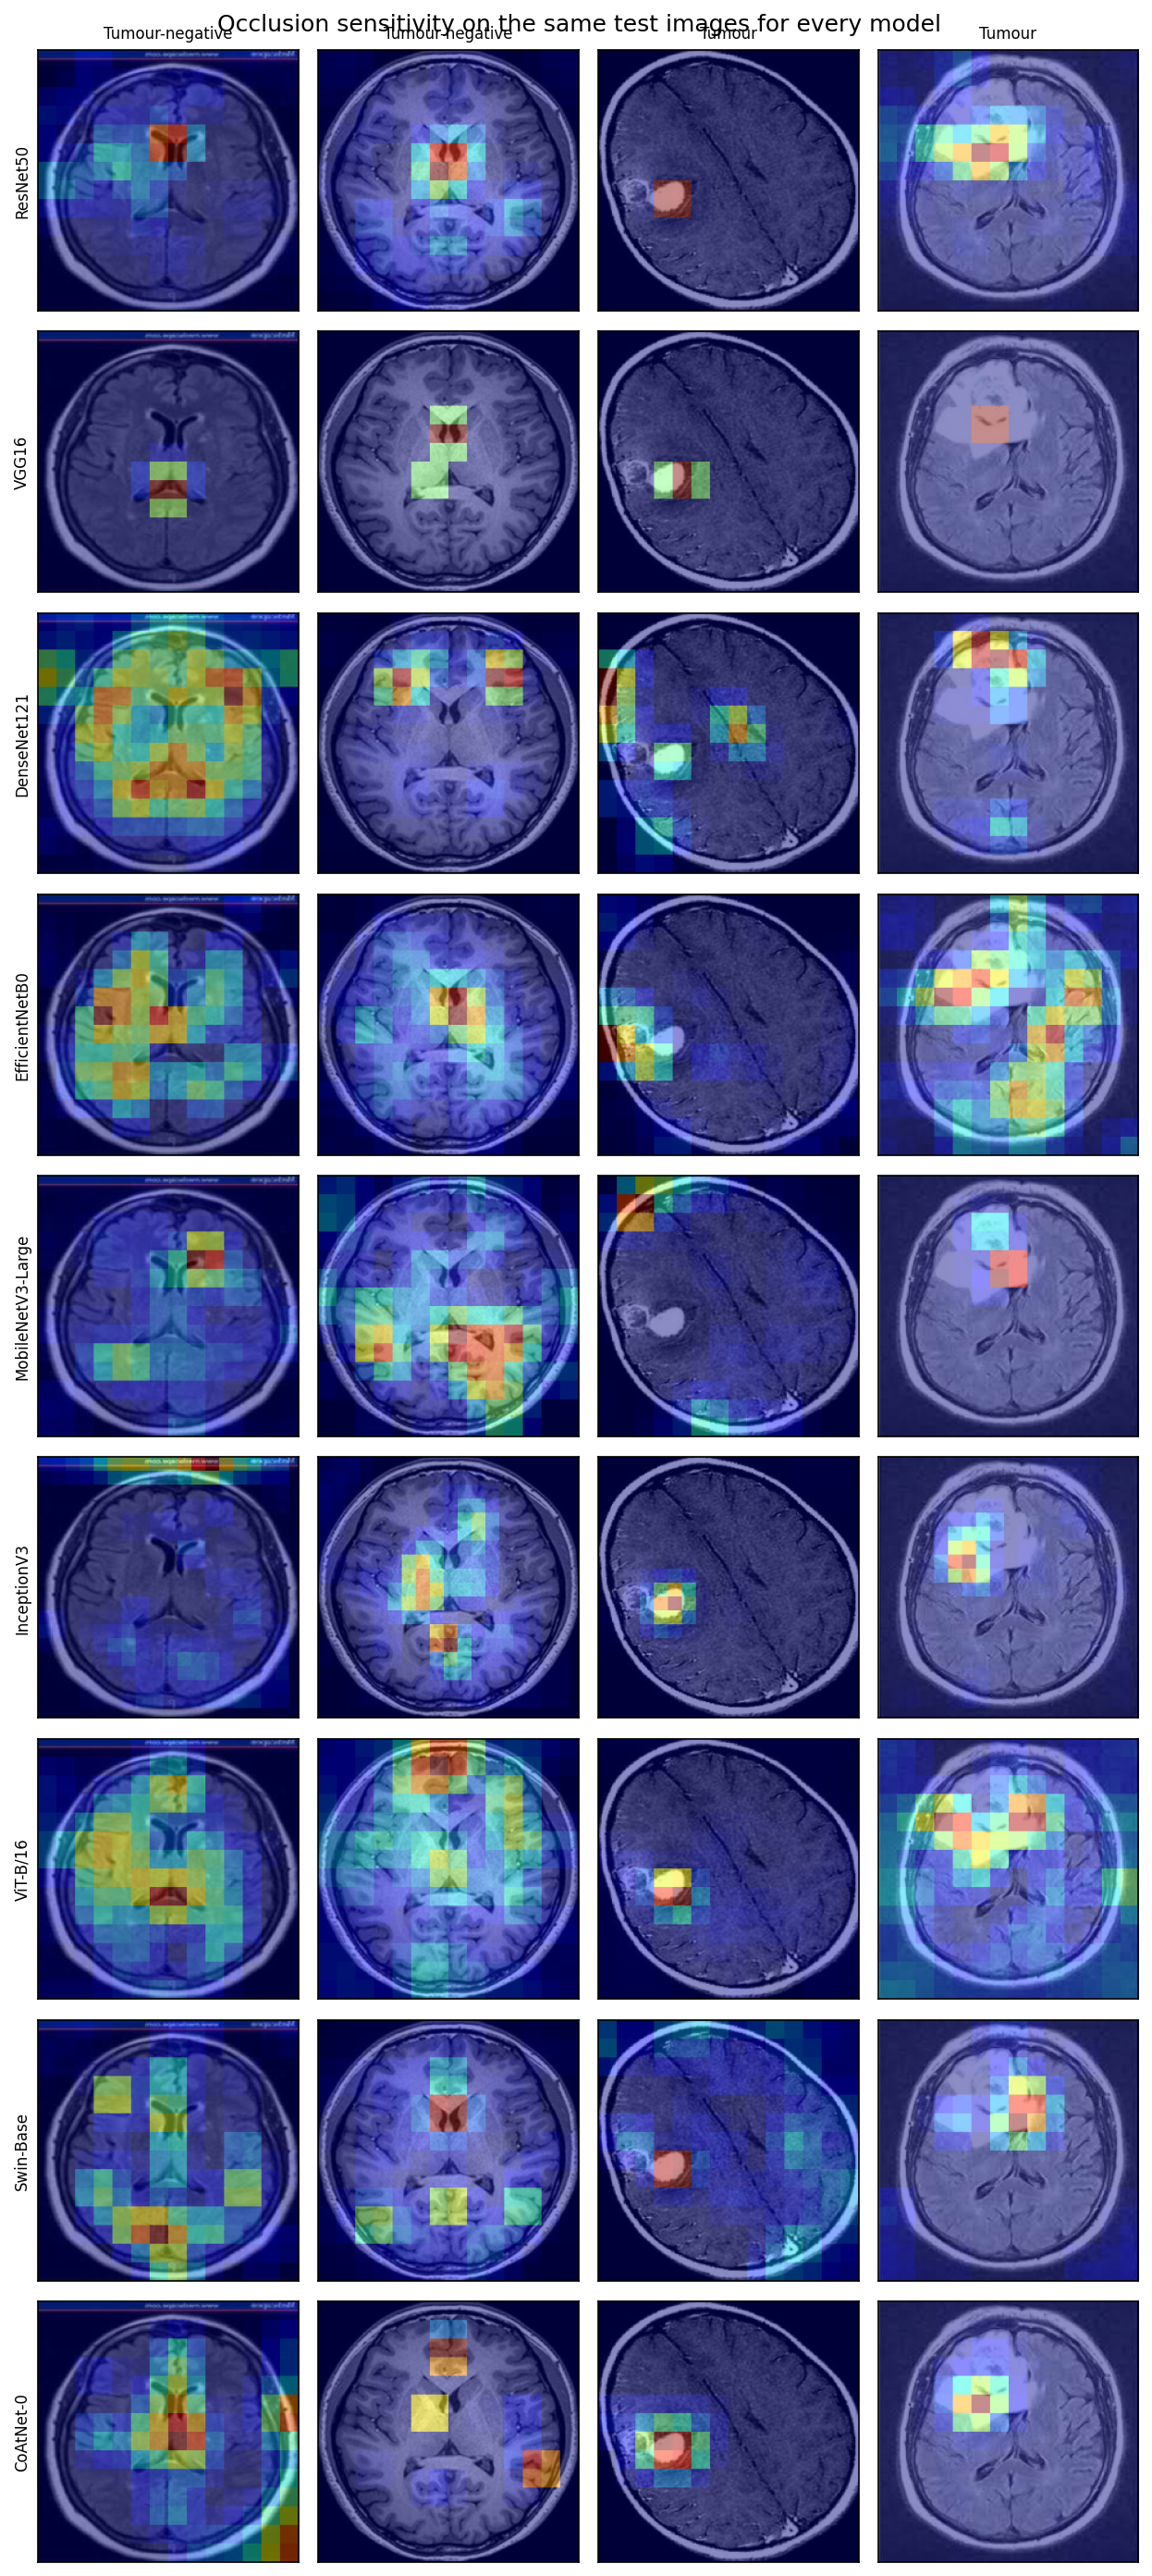
\includegraphics[width=\linewidth]{binary-detection/plots/15_occlusion_maps.png}
\caption{Binary detection: occlusion maps of every model on the same stratified test images.}
\end{figure}

\begin{figure}[htbp]
\centering
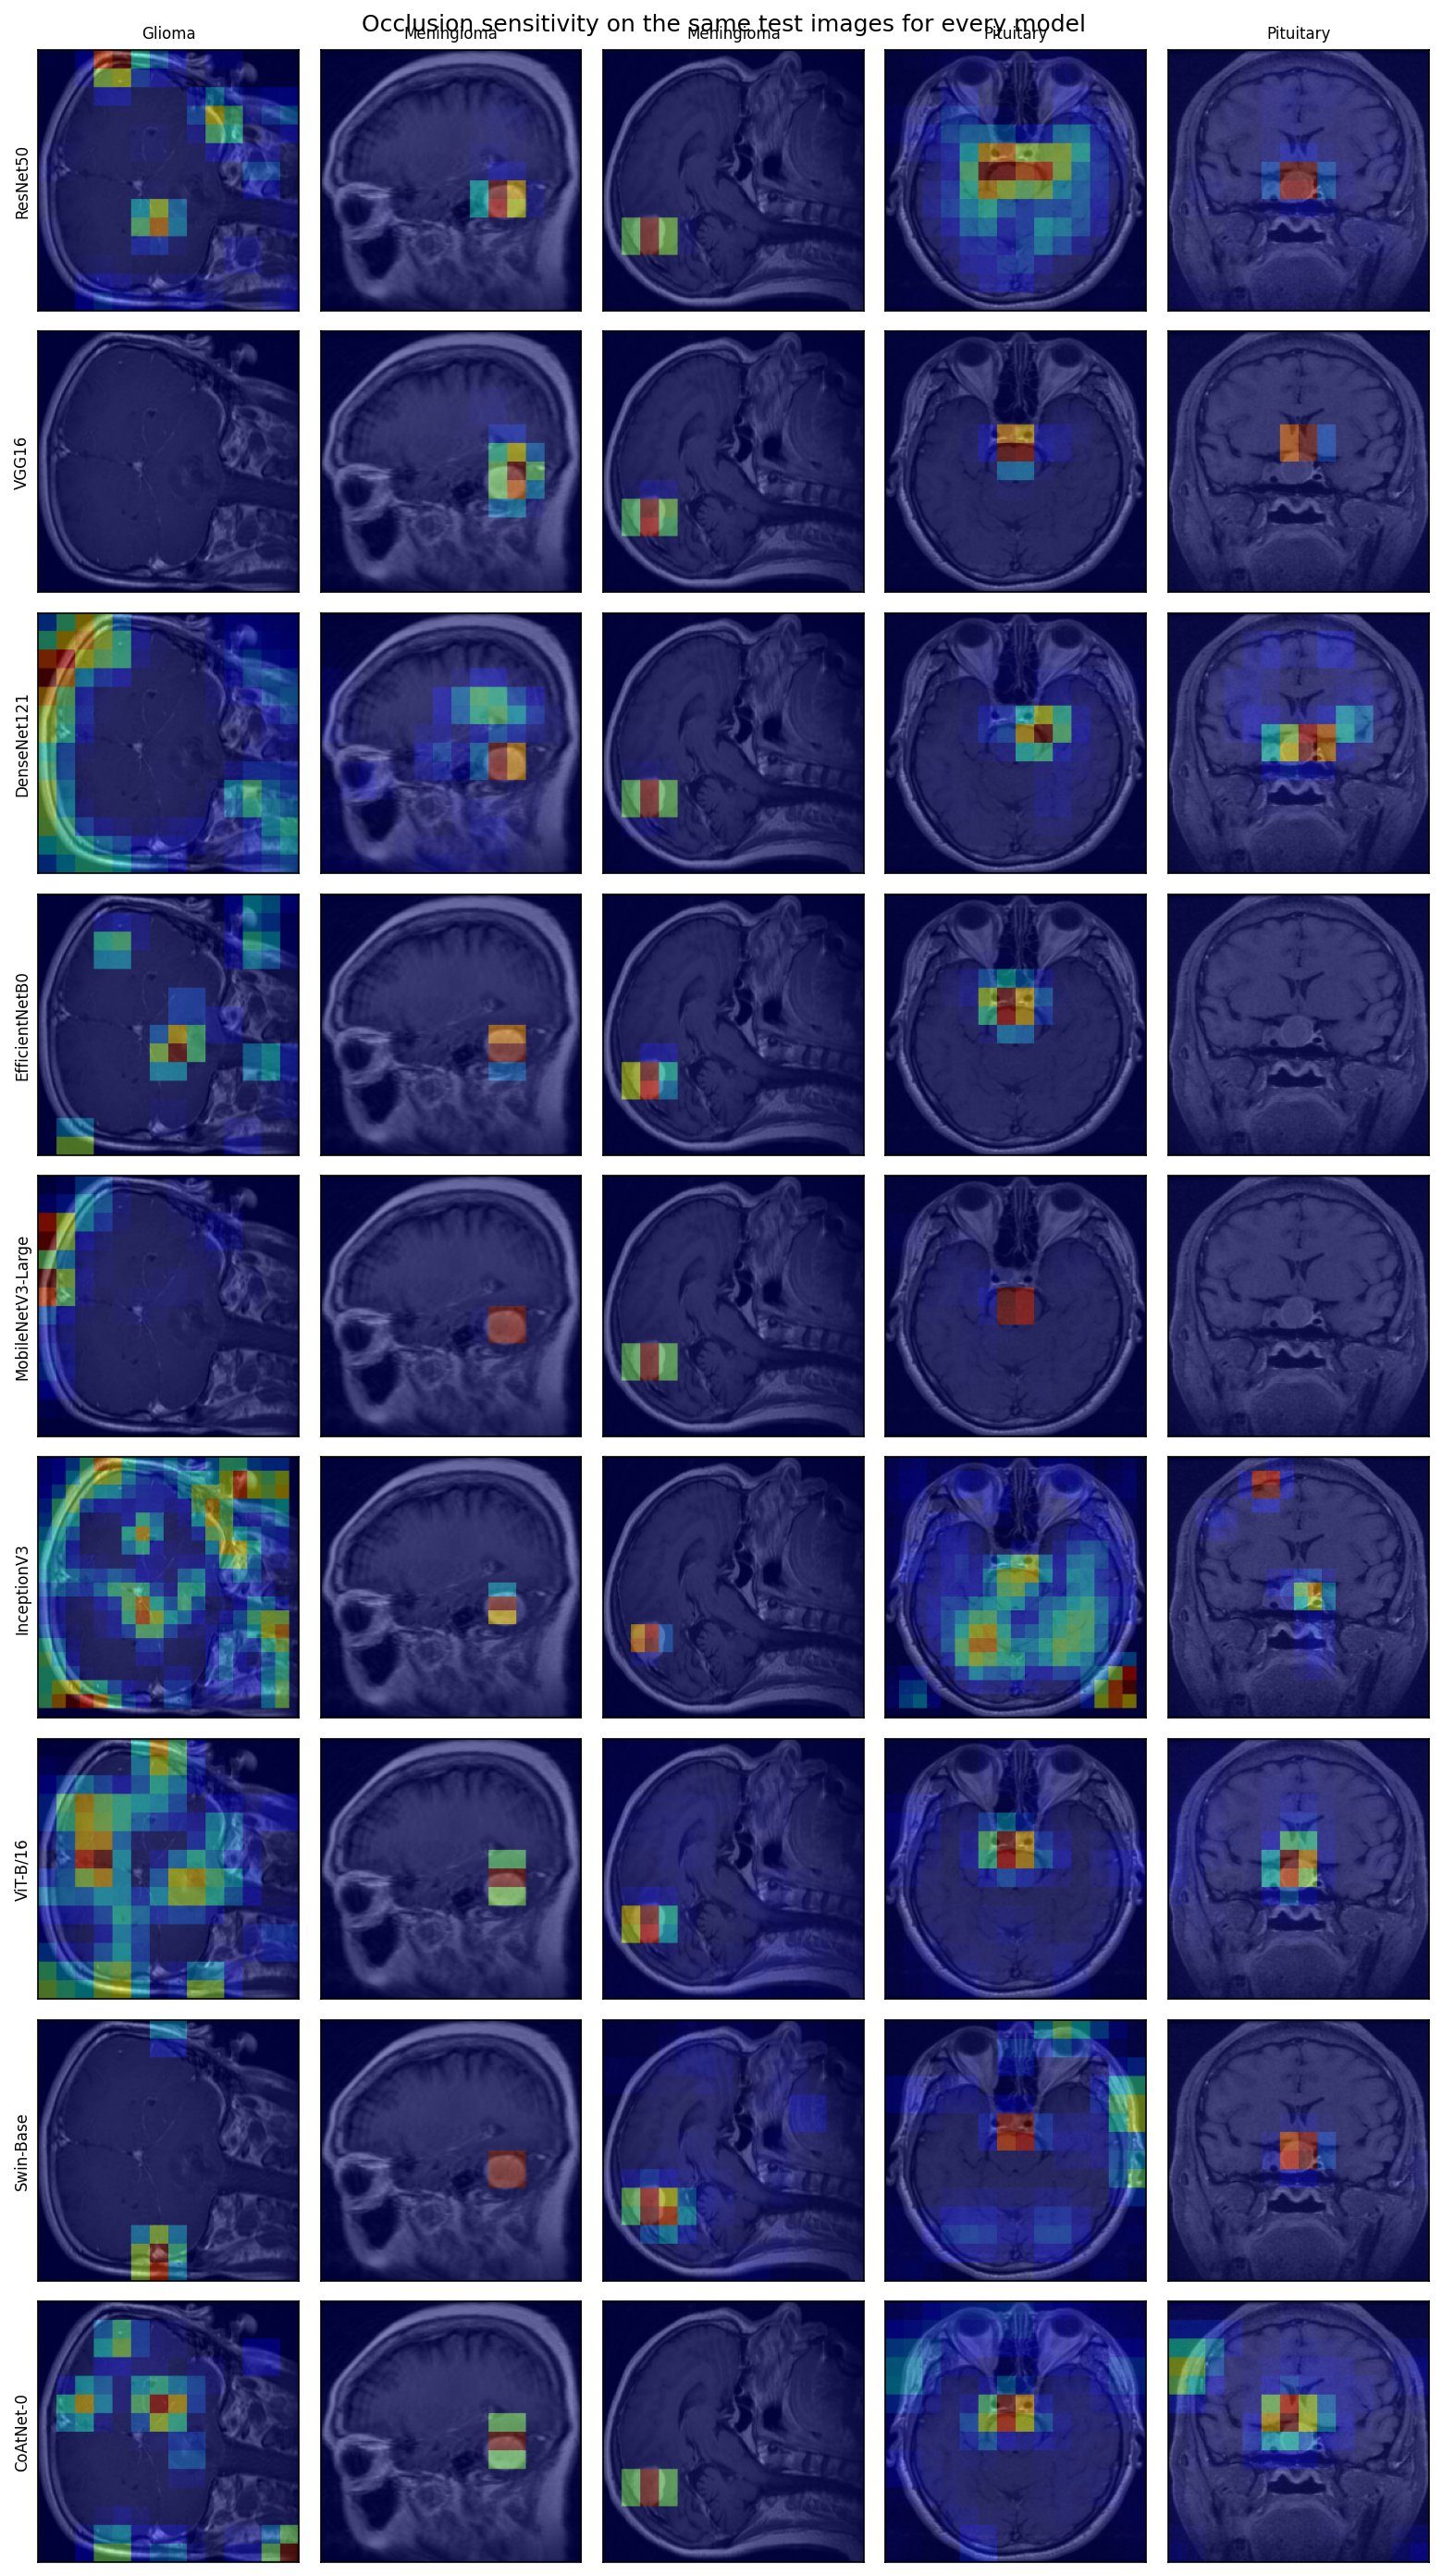
\includegraphics[width=\linewidth]{classification/plots/15_occlusion_maps.png}
\caption{Subtype classification: occlusion maps of every model on the same stratified test images.}
\end{figure}

\begin{figure}[htbp]
\centering
\panel{0.49}{binary-detection/plots/16_masking_test.png}{Binary detection.}\hfill
\panel{0.49}{classification/plots/16_masking_test.png}{Subtype classification.}
\caption{Masking test (inference only): test accuracy of each fold's checkpoint on full images, head-only images (background set to zero) and background-only images (head set to zero), mean $\pm$ standard deviation over folds.}
\end{figure}

\FloatBarrier
\section*{S6. Grad-CAM maps of every model}

\gradcamfigure{resnet50}{ResNet50}
\gradcamfigure{vgg16}{VGG16}
\gradcamfigure{densenet121}{DenseNet121}
\gradcamfigure{efficientnetb0}{EfficientNetB0}
\gradcamfigure{mobilenetv3-large}{MobileNetV3-Large}
\gradcamfigure{inceptionv3}{InceptionV3}
\gradcamfigure{vit-b-16}{ViT-B/16}
\gradcamfigure{swin-base}{Swin-Base}
\gradcamfigure{coatnet-0}{CoAtNet-0}

\end{document}
